\documentclass[tikz,border=10pt]{standalone}
\begin{document}
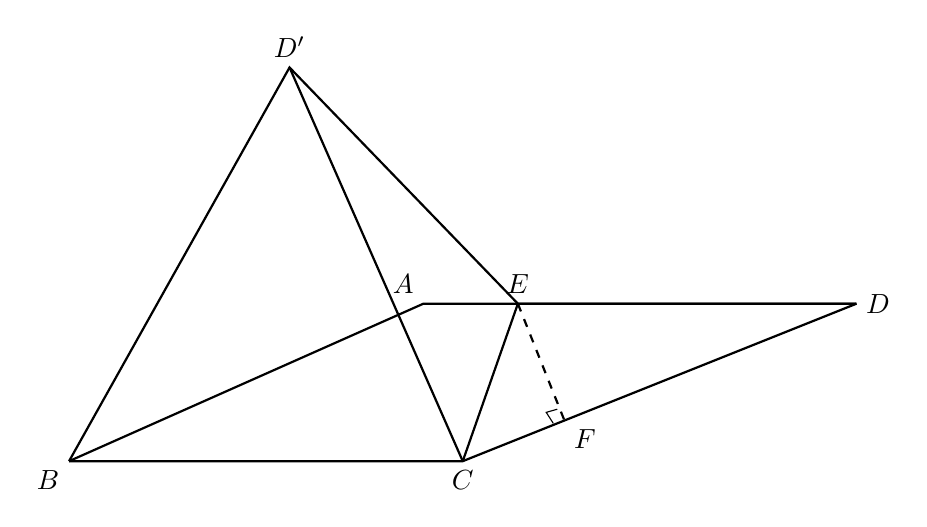
\begin{tikzpicture}[scale=1]
\coordinate (B) at (0,0);
\coordinate (C) at (5,0);
\coordinate (A) at (4.5,2);
\coordinate (D) at (10,2);
\coordinate (E) at (5.7,2);
\coordinate (D') at (2.8,5);
\coordinate (F) at (6.29,0.52);

\draw[thick] (B) -- (D') -- (E) -- (D);
\draw[thick] (B) -- (C) -- (D);
\draw[thick] (B) -- (A) -- (D);
\draw[thick] (D') -- (C);
\draw[thick] (C) -- (E);
\draw[dashed,thick] (E) -- (F);

% right angle mark at F between FE and FC
\draw (6.20,0.66) -- (6.06,0.62) -- (6.15,0.48);

\node[below left] at (B) {$B$};
\node[below] at (C) {$C$};
\node[above left] at (A) {$A$};
\node[right] at (D) {$D$};
\node[above] at (E) {$E$};
\node[above] at (D') {$D'$};
\node[below right] at (F) {$F$};
\end{tikzpicture}
\end{document}
